\chapter{Analiza i wyniki}\label{chap:analiza_i_wyniki}

W tym rozdziale przedstawiono szczegółową analizę oraz wyniki badań przeprowzadzonych w ramach przyjętej metodologii i kryteriów opisanych w rozdziale poprzednim. Przedstawione wyniki stanowią podstawę do sformułowania wniosków na temat charakterystyk badanych algorytmów oraz ich potencjalnych zastosowań w praktyce w dalszej części pracy. Dodatkowo, wnioski te mogą posłużyć jako wskazówki dla przyszłych badań nad optymalizacją i rozwijaniem algorytmów percepcji głębi, które będą w stanie sprostać coraz bardziej wymagającym zadaniom stawianym przez nowoczesne aplikacje wizyjne. W celu poprawienia przejrzystości analizy, na wykresach algorytmy testowane na zbiorze który brał udział w procesie uczenia zostały specjalnie oznaczone.

\section{Dokładność estymacji}
\subsection{Dokładność progowa}
Dokładność progowa to miara używana do oceny wydajności estymacji głębokości przez modele sztucznej inteligencji. Mierzy ona odsetek oszacowań głębokości, które mieszczą się w określonym z góry progu względem wartości rzeczywistych. Konkretnie, oblicza procent przewidywanych głębokości, które spełniają warunek przedstawiony we wzorze \ref{eq:4}. Metryka ta jest szczególnie użyteczna do oceny, jak blisko przewidywane głębokości są do wartości zmierzonych w określonym poziomie tolerancji. Założony podczas niniejszej analizy progi to $1,25$ oraz kwadrat i sześcian tej wartości. Pozwoli to na bardziej szczegółową ocenę modeli w sytuacjach, gdzie dokładne wartości są trudne do przewidzenia, ale bliskie przybliżenia są nadal wartościowe. Każda z analizowanych metod została uruchomiona na siedmiu zbiorach danych opisanych w rozdziale \ref{chap:przedstawienie_zastosowanych_narzędzi}, wyniki uruchomień zostały zestawione z rzeczywistymi mapami głębi, a następnie wyliczone zostały dokładności progowe, które zaprezentowane zostały poprzez wykresy znajdujące się na następnych stronach.

\begin{figure}[H]
    \centering
    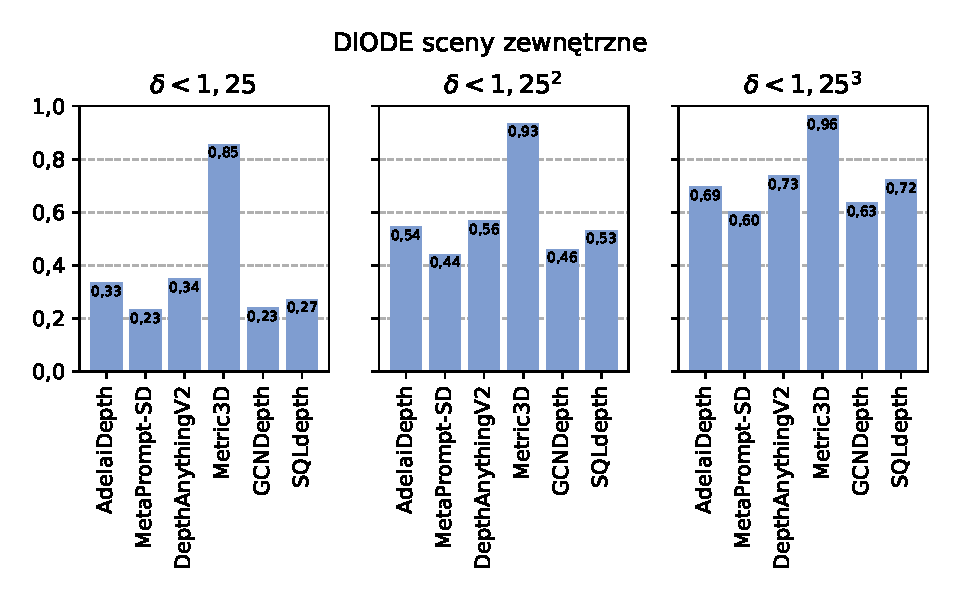
\includegraphics{plots/delta/0}
    \caption{Wyniki dokładności progowej na zbiorze DIODE na części ze scenami zewnętrznymi.}
    \label{fig:delta_0}
\end{figure}
\begin{figure}[H]
    \centering
    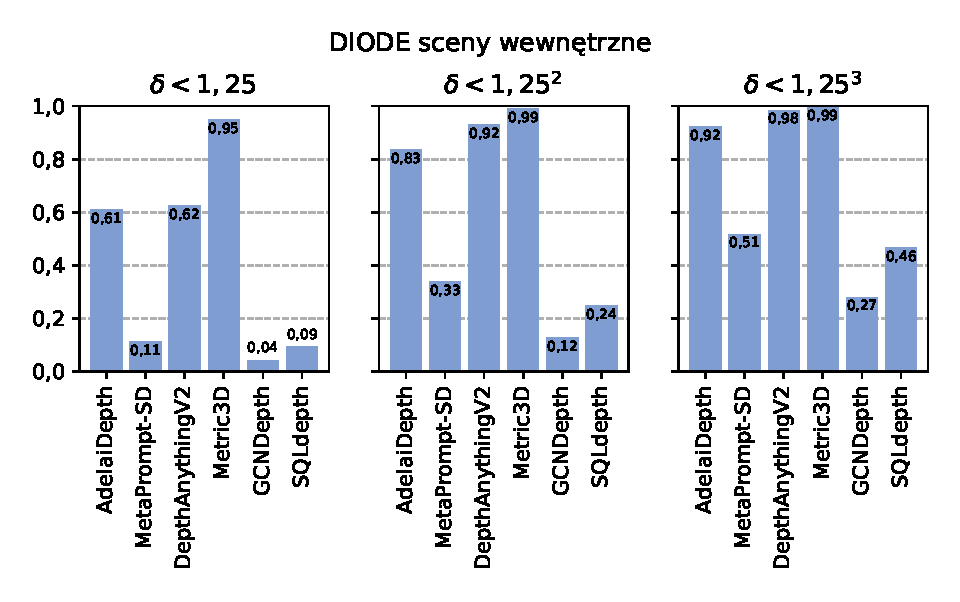
\includegraphics{plots/delta/1}
    \caption{Wyniki dokładności progowej na zbiorze DIODE na części ze scenami wewnętrznymi.}
    \label{fig:delta_1}
\end{figure}
\begin{figure}[H]
    \centering
    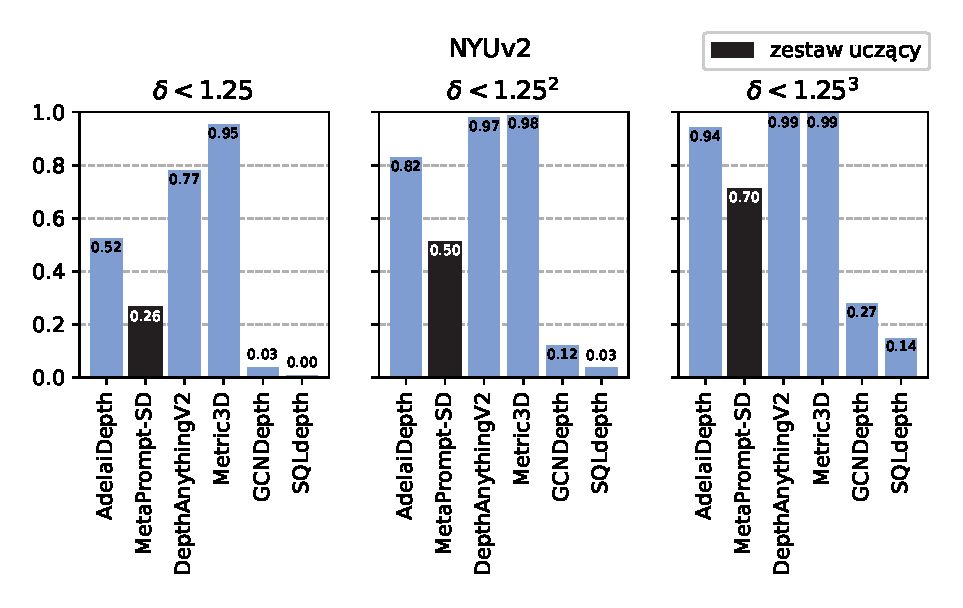
\includegraphics{plots/delta/2}
    \caption{Wyniki dokładności progowej na zbiorze NYUv2.}
    \label{fig:delta_2}
\end{figure}
\begin{figure}[H]
    \centering
    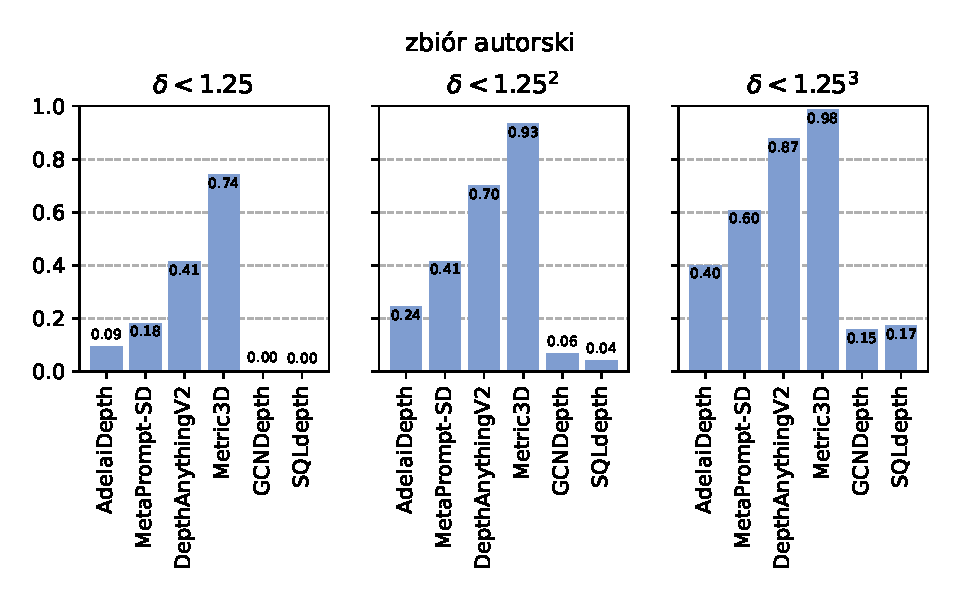
\includegraphics{plots/delta/3}
    \caption{Wyniki dokładności progowej na zbiorze autorskim.}
    \label{fig:delta_3}
\end{figure}
\begin{figure}[H]
    \centering
    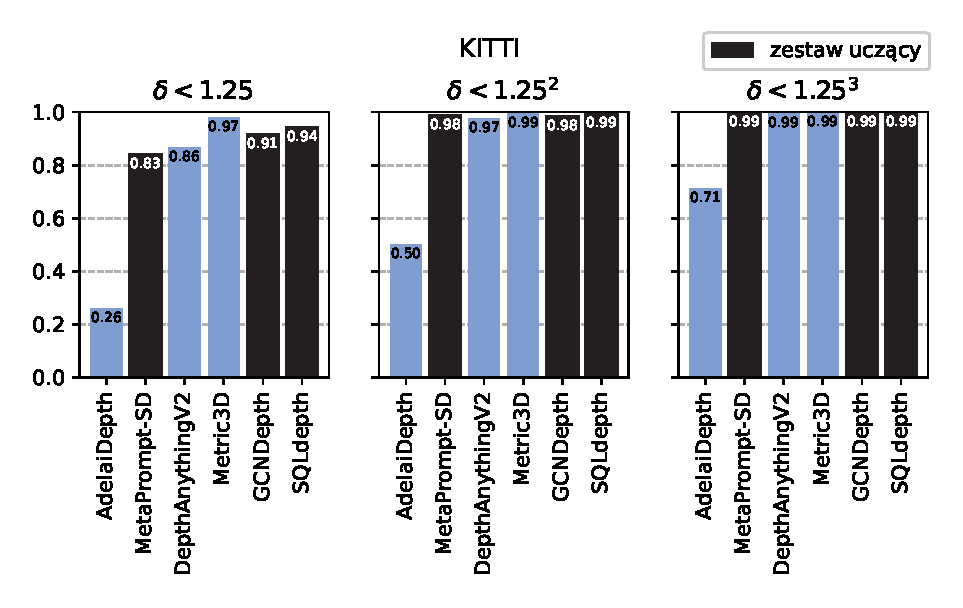
\includegraphics{plots/delta/4}
    \caption{Wyniki dokładności progowej na zbiorze KITTI.}
    \label{fig:delta_4}
\end{figure}
\begin{figure}[H]
    \centering
    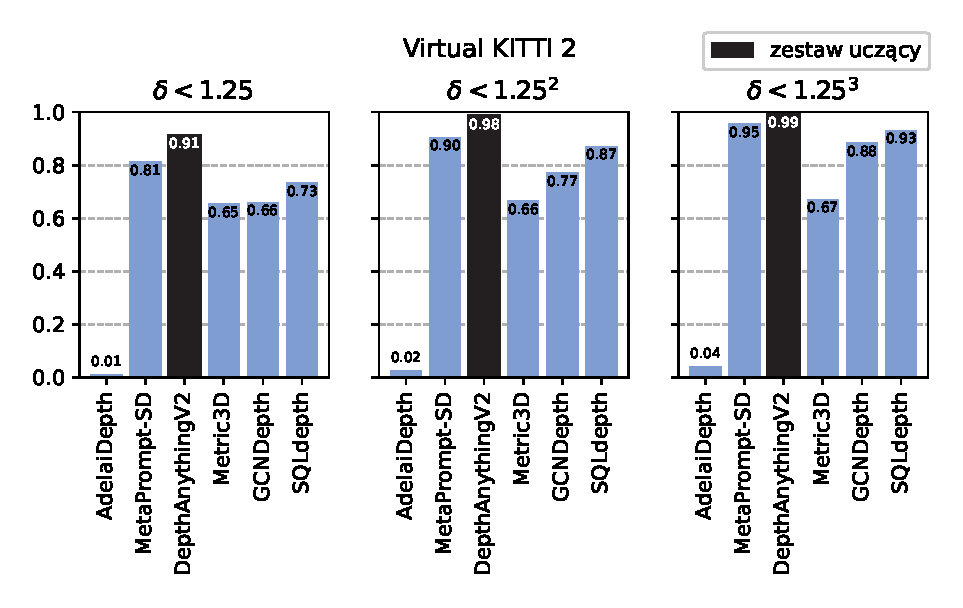
\includegraphics{plots/delta/5}
    \caption{Wyniki dokładności progowej na zbiorze Virtual KITTI 2.}
    \label{fig:delta_5}
\end{figure}
\begin{figure}[H]
    \centering
    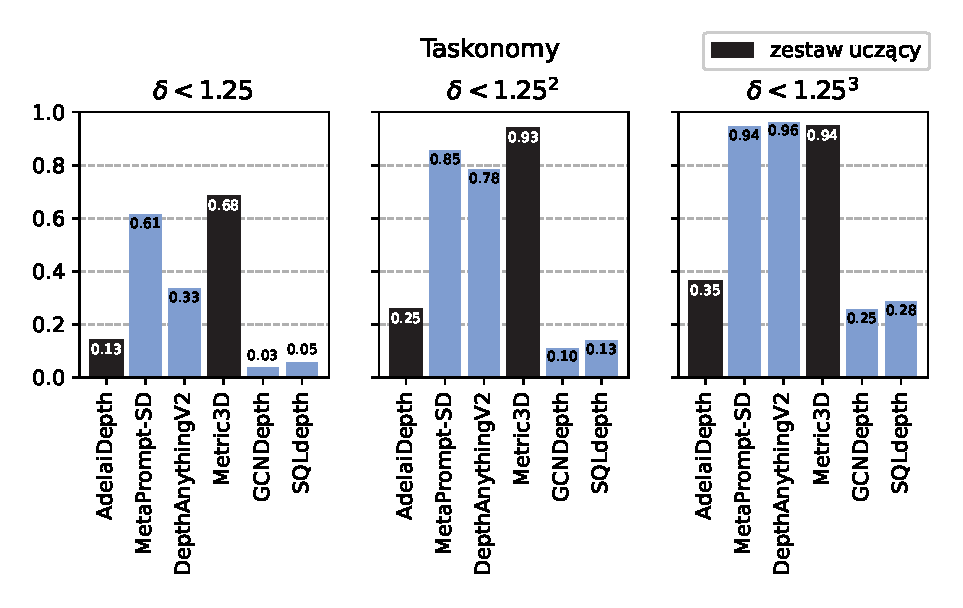
\includegraphics{plots/delta/6}
    \caption{Wyniki dokładności progowej na zbiorze Taskonomy.}
    \label{fig:delta_6}
\end{figure}

\subsection{Średni procentowy błąd bezwzględny}
Sekcja ta zawiera wyniki osiągnięte przez analizowane algorytmy w dziedzinie średniego bezwzględnego błedu estymacji \ref{eq:2}. Jest to metryka oznaczająca średnią procentową bezwzlęgną różnicę między wartościami, które są dopasowane przez algorytm, a wartościami danych rzeczywistych. Metryka ta uznawana jest za najbardziej uniwersalną, z tego powodu najczęściej występuje w publikacjach naukowych dotyczących omawianych algorytmów. W tym podrozdziale znajdują się wykresy sporządzone na podstawie wyników uruchomień algorytmów na założonych zestawach danych. Z uruchomienia na zestawie syntetycznych danych Virtual KITTI 2 został wyłączony algorytm AdelaiDepth, ze względu na bardzo niekorzystny wynik\footnote{Algorytm AdelaiDepth na wirtualnym zbiorze Virtual KITTI 2 uzyskał wynik powyżej 1000\% AbsRel}. Metoda ta została nauczona na zestawie danych przedstawiających sceny wyłącznie wewnętrzne i realistyczne, stąd aby zachować przejrzystość wizualizacji zdecydowano się na taki zabieg.

\begin{figure}[H]
    \centering
    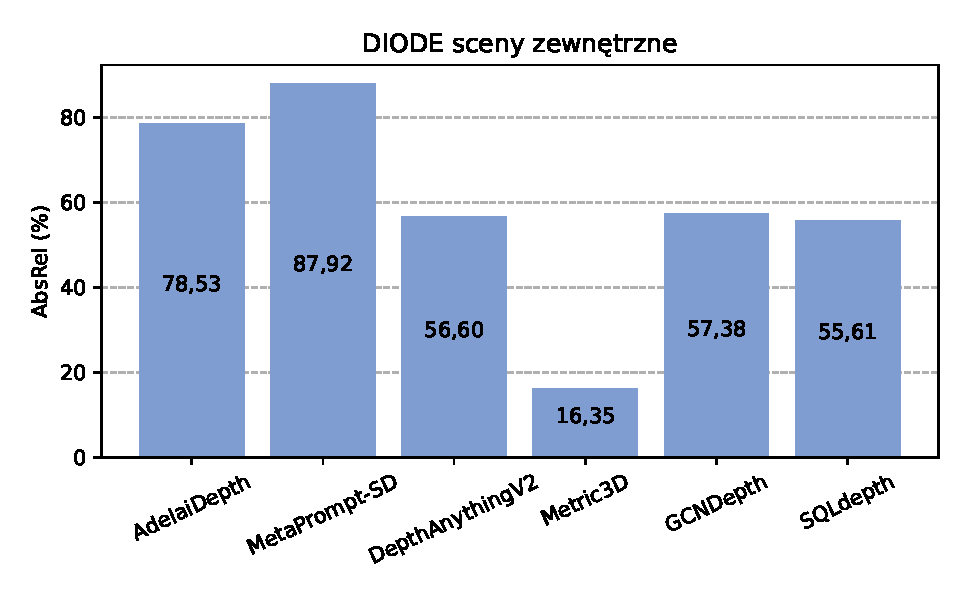
\includegraphics{plots/absrel/0}
    \caption{Średni bezwzględny błąd procentowy na zbiorze DIODE na części ze scenami zewnętrznymi.}
    \label{fig:absrel_0}
\end{figure}
\begin{figure}[H]
    \centering
    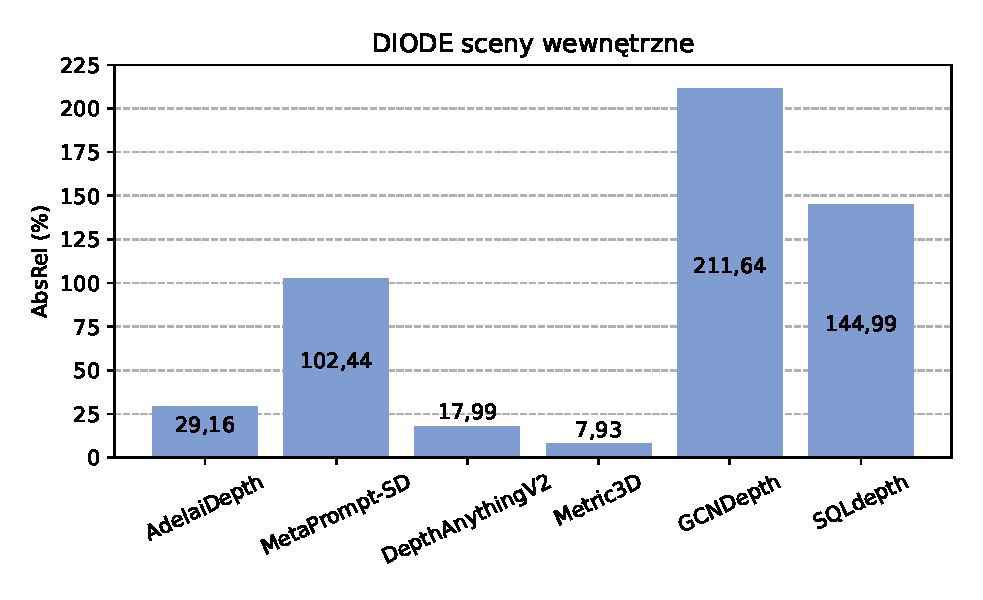
\includegraphics{plots/absrel/1}
    \caption{Średni bezwzględny błąd procentowy na zbiorze DIODE na części ze scenami wewnętrznymi.}
    \label{fig:absrel_1}
\end{figure}
\begin{figure}[H]
    \centering
    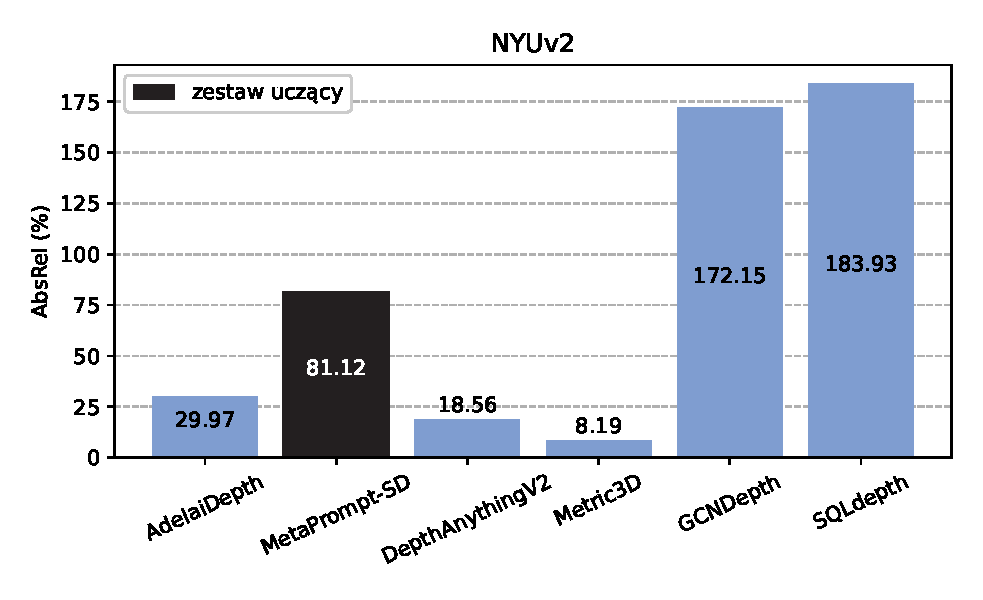
\includegraphics{plots/absrel/2}
    \caption{Średni bezwzględny błąd procentowy na zbiorze NYUv2.}
    \label{fig:absrel_2}
\end{figure}
\begin{figure}[H]
    \centering
    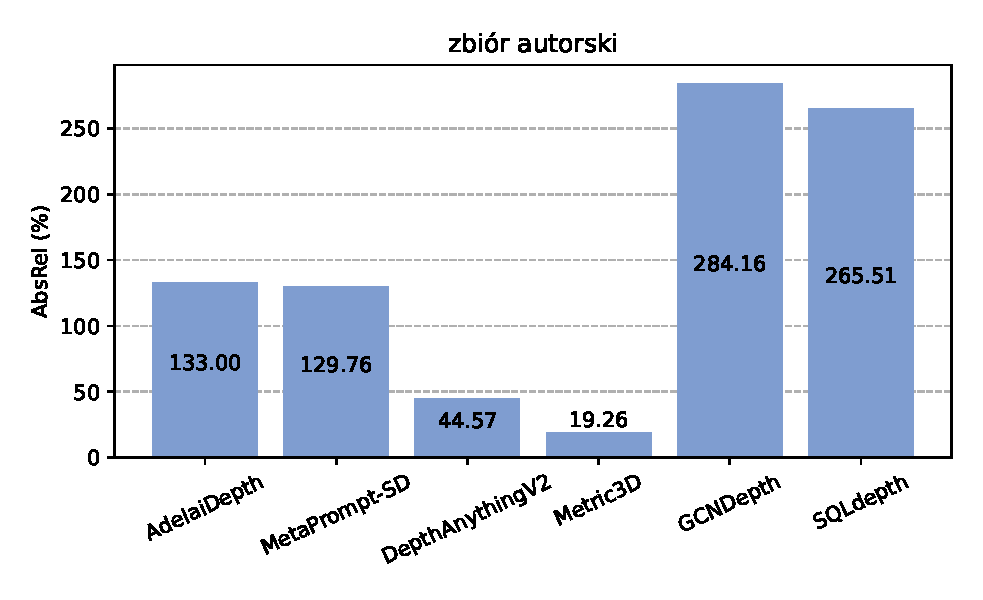
\includegraphics{plots/absrel/3}
    \caption{Średni bezwzględny błąd procentowy na zbiorze autorskim.}
    \label{fig:absrel_3}
\end{figure}
\begin{figure}[H]
    \centering
    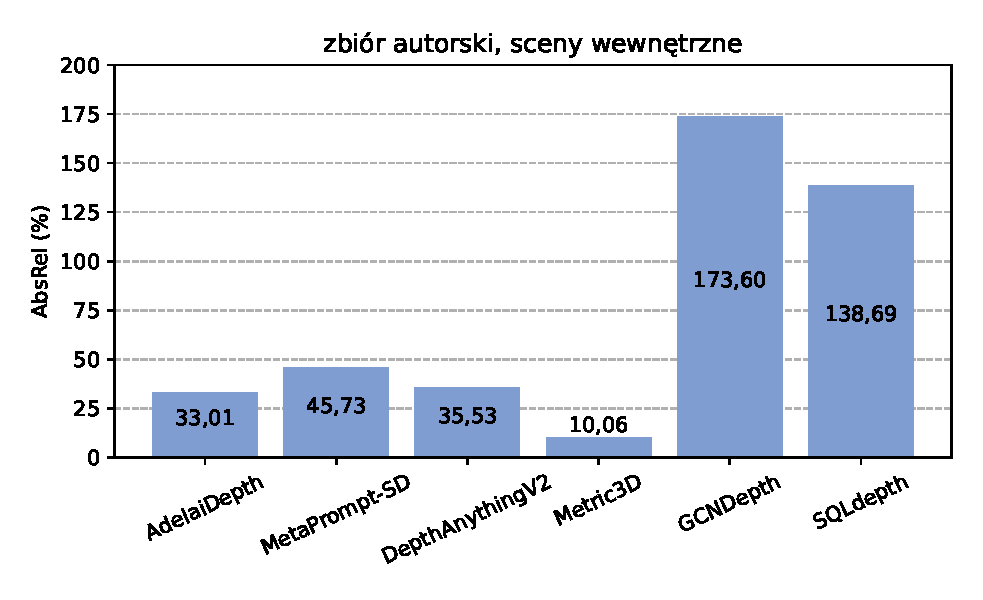
\includegraphics{plots/absrel/4}
    \caption{Średni bezwzględny błąd procentowy na zbiorze KITTI.}
    \label{fig:absrel_4}
\end{figure}
\begin{figure}[H]
    \centering
    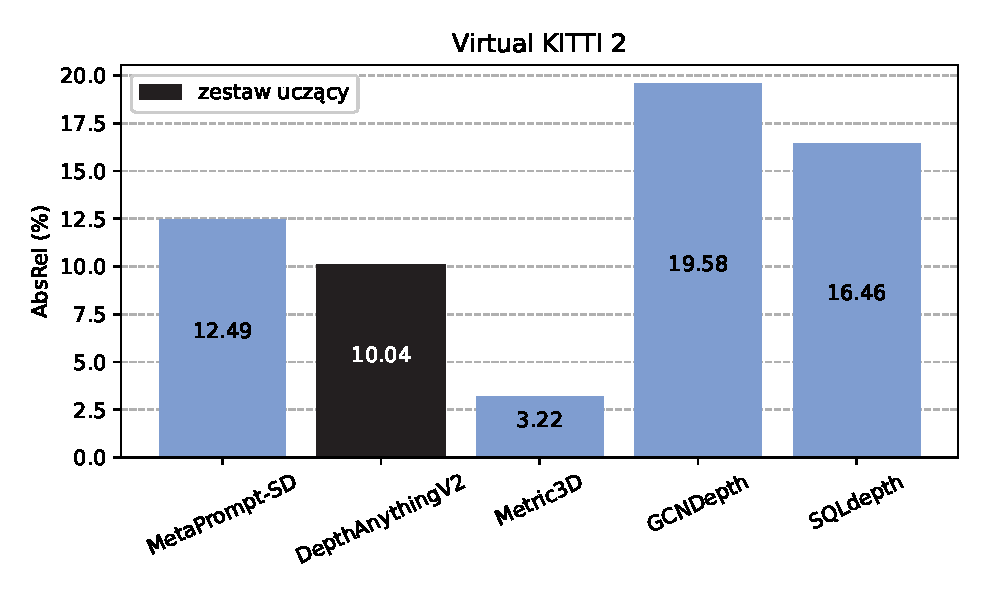
\includegraphics{plots/absrel/5}
    \caption{Średni bezwzględny błąd procentowy na zbiorze Virtual KITTI 2.}
    \label{fig:absrel_5}
\end{figure}
\begin{figure}[H]
    \centering
    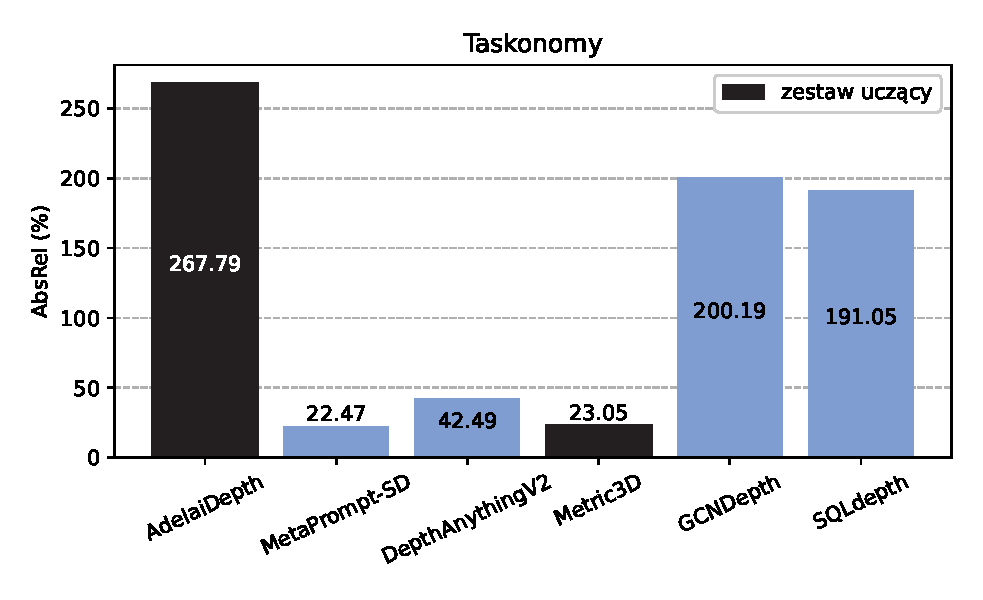
\includegraphics{plots/absrel/6}
    \caption{Średni bezwzględny błąd procentowy na zbiorze Taskonomy.}
    \label{fig:absrel_6}
\end{figure}

\subsection{Pierwiastek błędu średniokwadratowego}
Ostatnim analizowanym współczynnikiem oceny dokładności prognozy jest pierwiastek błędu średniokwadratowego \ref{eq:3}. Oznacza on średnią różnicę między wartością przewidywaną a rzeczywistą na obrazach z danego zbioru danych, z czego wynika rzetelne odzwierciedlenie dokładności algorytmu. Jest to natomiast metryka bardziej bezwzględna niż wartość średniego procentowego błędu bezwzględnego. Wyniki analizy przedstawiają następujące wykresy.

\begin{figure}[H]
    \centering
    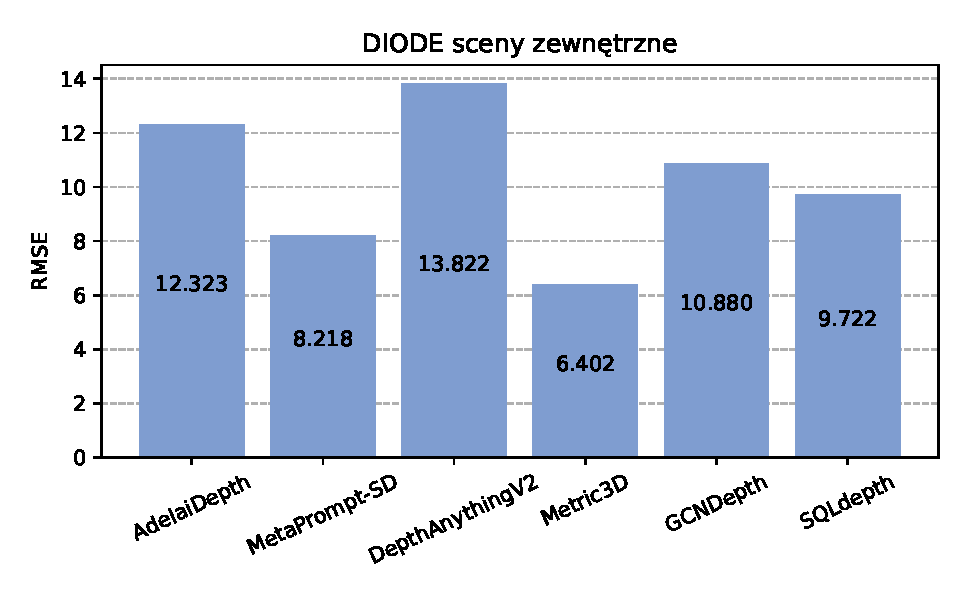
\includegraphics{plots/rmse/0}
    \caption{Pierwiastek błędu średniokwadratowego uzyskany na zbiorze DIODE na części ze scenami zewnętrznymi.}
    \label{fig:rmse_0}
\end{figure}
\begin{figure}[H]
    \centering
    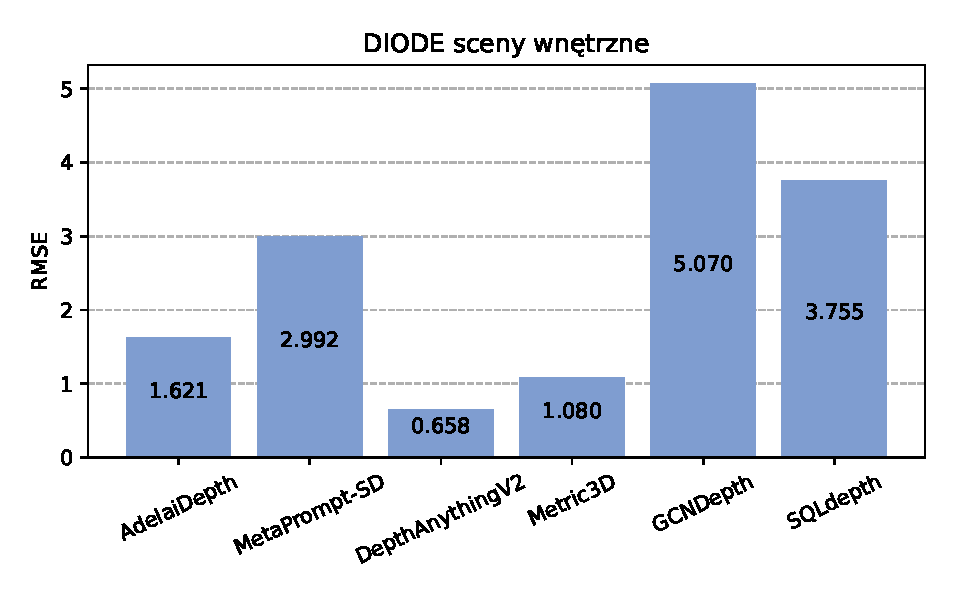
\includegraphics{plots/rmse/1}
    \caption{Pierwiastek błędu średniokwadratowego uzyskany na zbiorze DIODE na części ze scenami wewnętrznymi.}
    \label{fig:rmse_1}
\end{figure}
\begin{figure}[H]
    \centering
    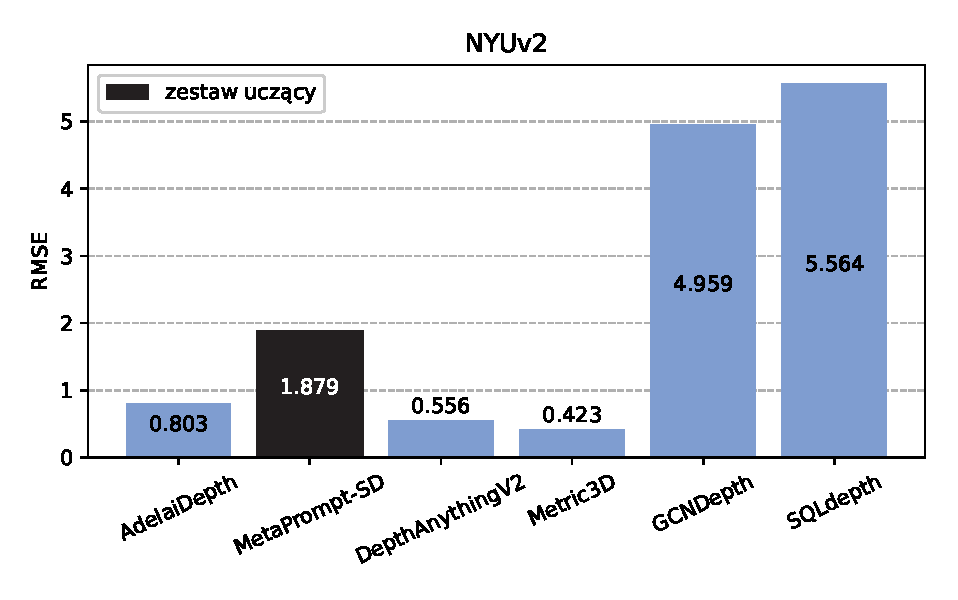
\includegraphics{plots/rmse/2}
    \caption{Pierwiastek błędu średniokwadratowego uzyskany na zbiorze NYUv2.}
    \label{fig:rmse_2}
\end{figure}
\begin{figure}[H]
    \centering
    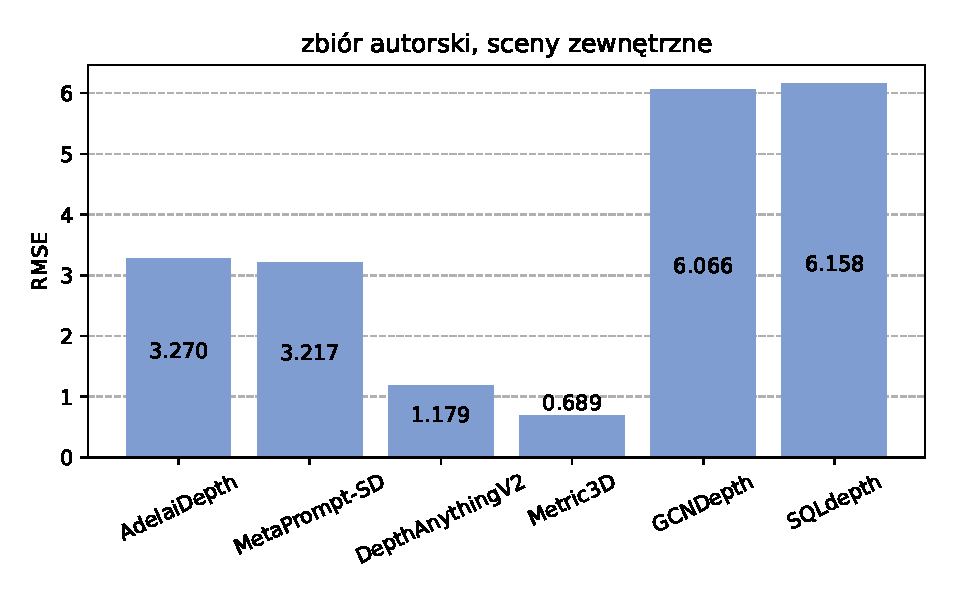
\includegraphics{plots/rmse/3}
    \caption{Pierwiastek błędu średniokwadratowego uzyskany na zbiorze autorskim.}
    \label{fig:rmse_3}
\end{figure}
\begin{figure}[H]
    \centering
    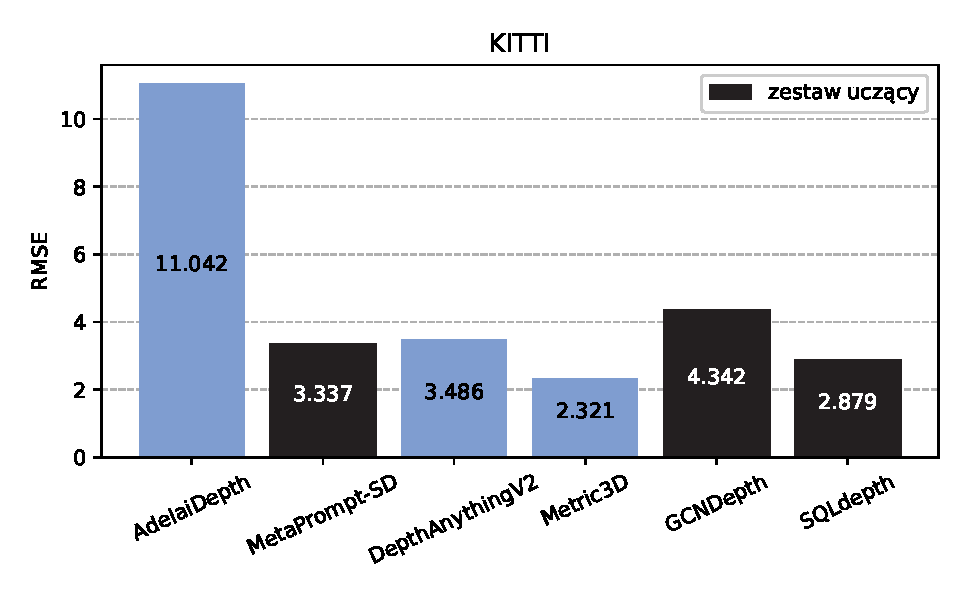
\includegraphics{plots/rmse/4}
    \caption{Pierwiastek błędu średniokwadratowego uzyskany na zbiorze KITTI.}
    \label{fig:rmse_4}
\end{figure}
\begin{figure}[H]
    \centering
    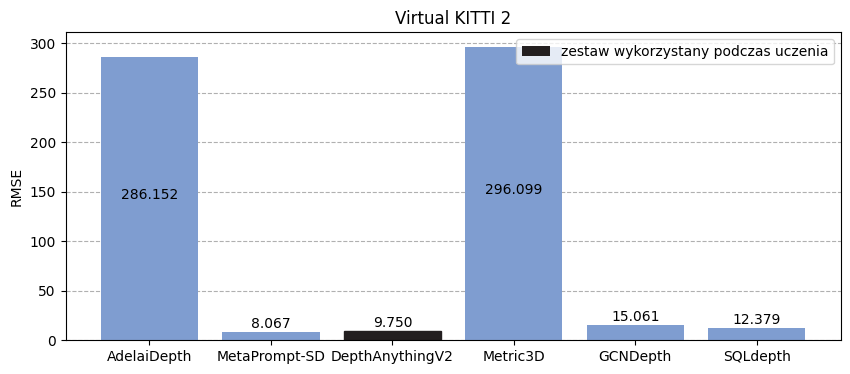
\includegraphics{plots/rmse/5}
    \caption{Pierwiastek błędu średniokwadratowego uzyskany na zbiorze Virtual KITTI 2.}
    \label{fig:rmse_5}
\end{figure}
\begin{figure}[H]
    \centering
    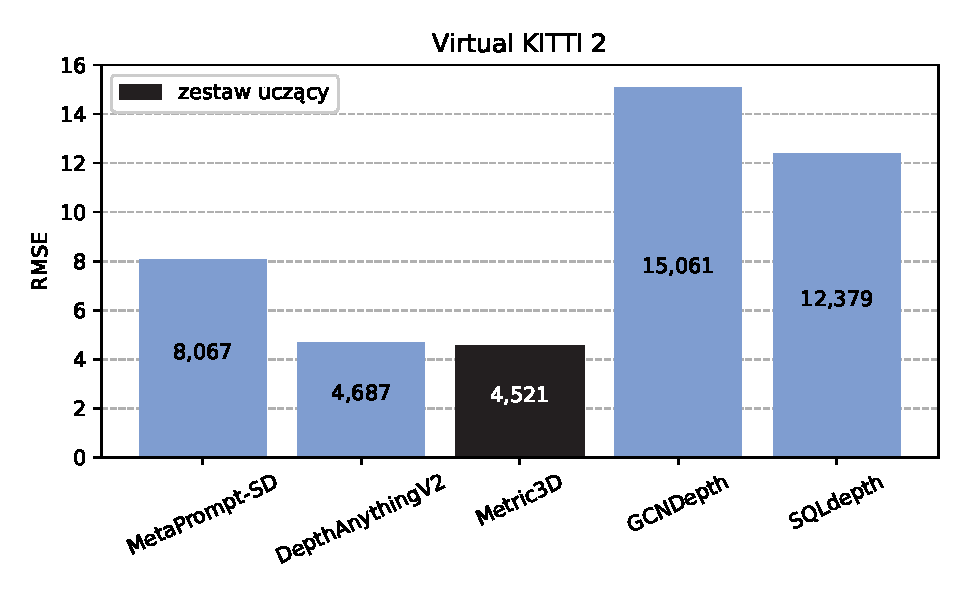
\includegraphics{plots/rmse/6}
    \caption{Pierwiastek błędu średniokwadratowego uzyskany na zbiorze Taskonomy.}
    \label{fig:rmse_6}
\end{figure}


\section{Czas realizacji pojedynczej estymacji}
Podczas analizy algorytmów w dziedzinie ich dokładności zostały również zebrane informacje na temat czasu wymaganego przez algorytm do wykonania estymacji głębi na pojedynczym obrazie. W czas ten wlicza się wczytanie obrazu, dokonanie predykcji i ewentualne skalowanie mapy głębi (w zależności od algorytmu). Uśrednione wyniki przedstawione zostały w postaci poniższych wykresów.
\begin{figure}[H]
    \centering
    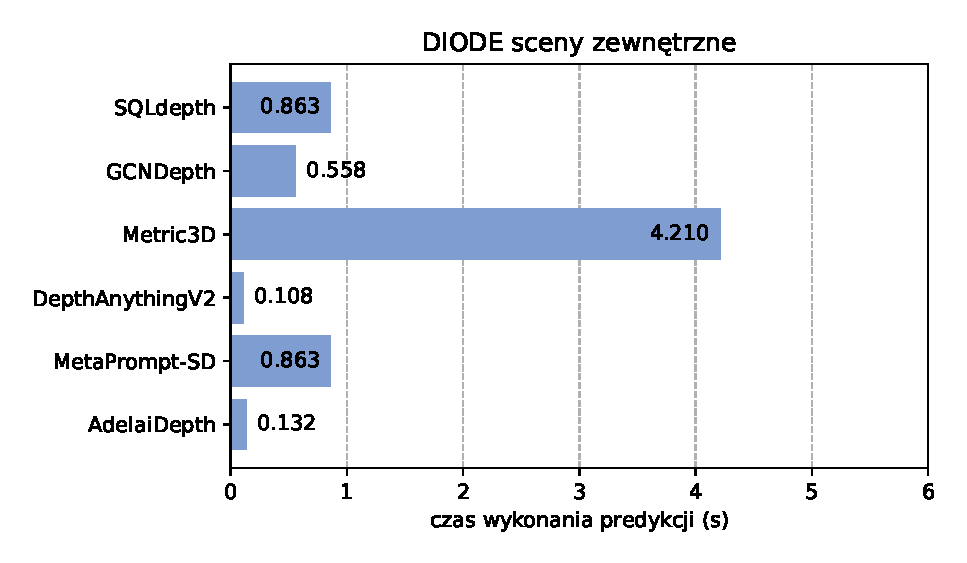
\includegraphics{plots/exec_time/0}
    \caption{Średni czas wykonania estymacji na zbiorze DIODE na części ze scenami zewnętrznymi.}
    \label{fig:exec_time_0}
\end{figure}
\begin{figure}[H]
    \centering
    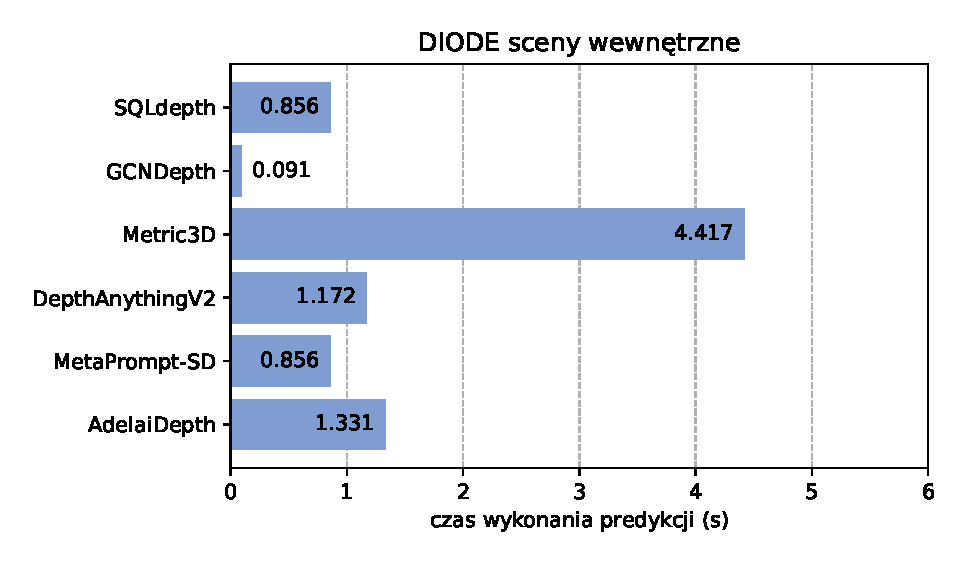
\includegraphics{plots/exec_time/1}
    \caption{Średni czas wykonania estymacji na zbiorze DIODE na części ze scenami wewnętrznymi.}
    \label{fig:exec_time_1}
\end{figure}
\begin{figure}[H]
    \centering
    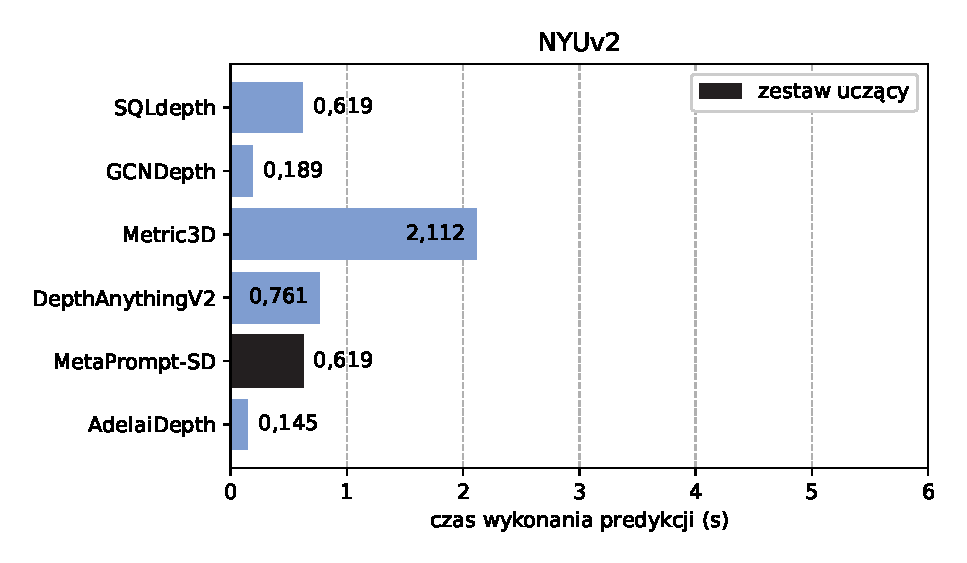
\includegraphics{plots/exec_time/2}
    \caption{Średni czas wykonania estymacji na zbiorze NYUv2.}
    \label{fig:exec_time_2}
\end{figure}
\begin{figure}[H]
    \centering
    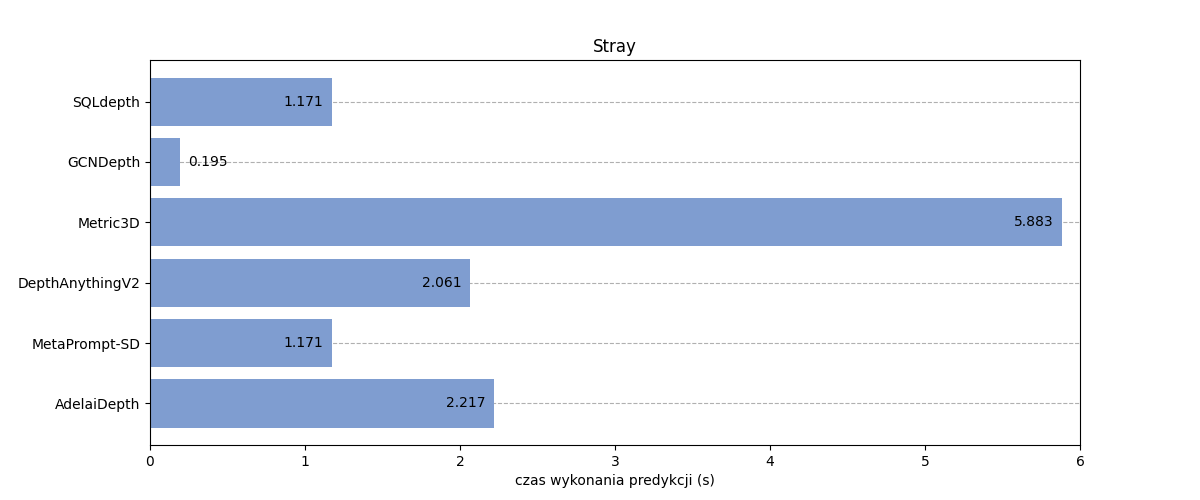
\includegraphics{plots/exec_time/3}
    \caption{Średni czas wykonania estymacji na zbiorze autorskim.}
    \label{fig:exec_time_3}
\end{figure}
\begin{figure}[H]
    \centering
    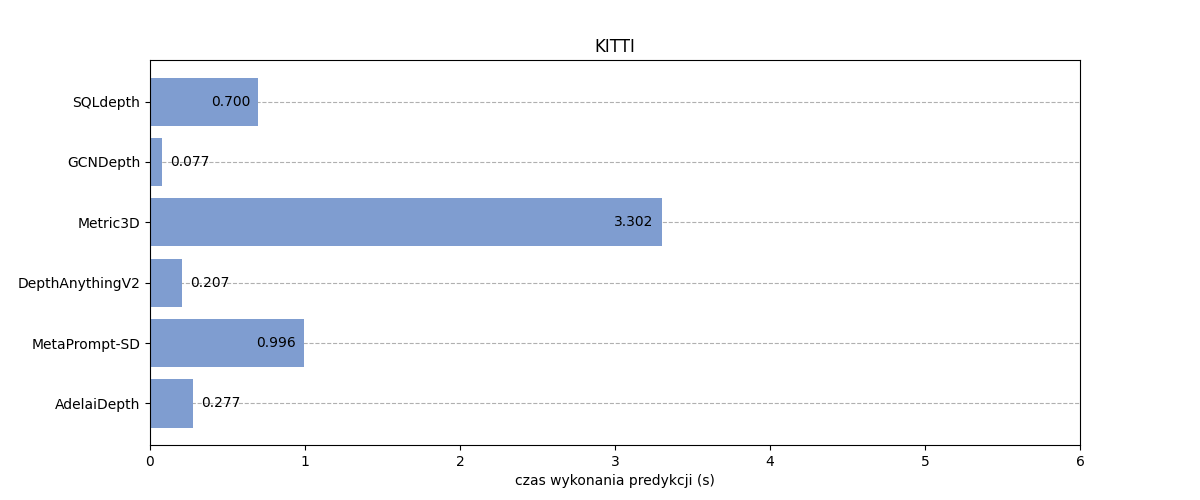
\includegraphics{plots/exec_time/4}
    \caption{Średni czas wykonania estymacji na zbiorze KITTI.}
    \label{fig:exec_time_4}
\end{figure}
\begin{figure}[H]
    \centering
    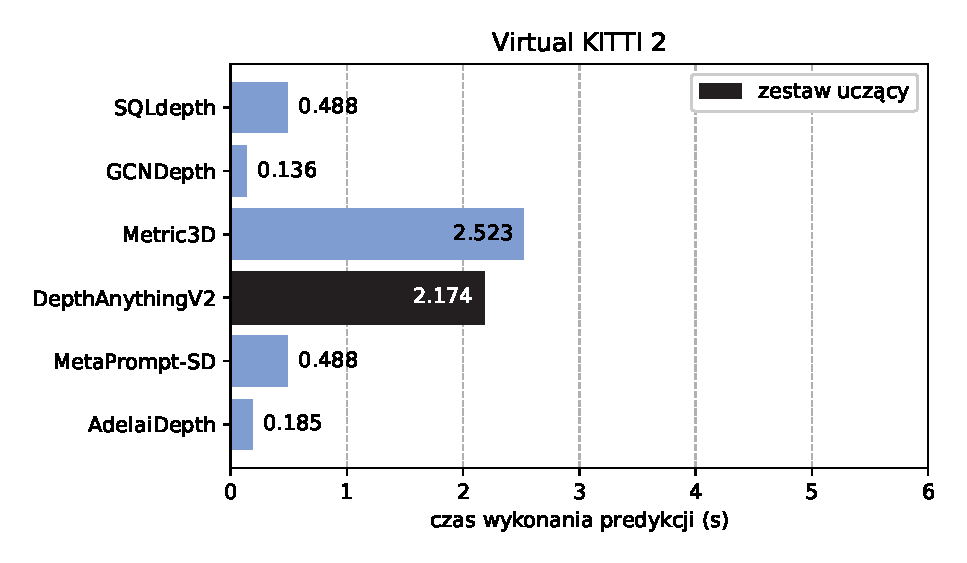
\includegraphics{plots/exec_time/5}
    \caption{Średni czas wykonania estymacji na zbiorze Virtual KITTI 2.}
    \label{fig:exec_time_5}
\end{figure}
\begin{figure}[H]
    \centering
    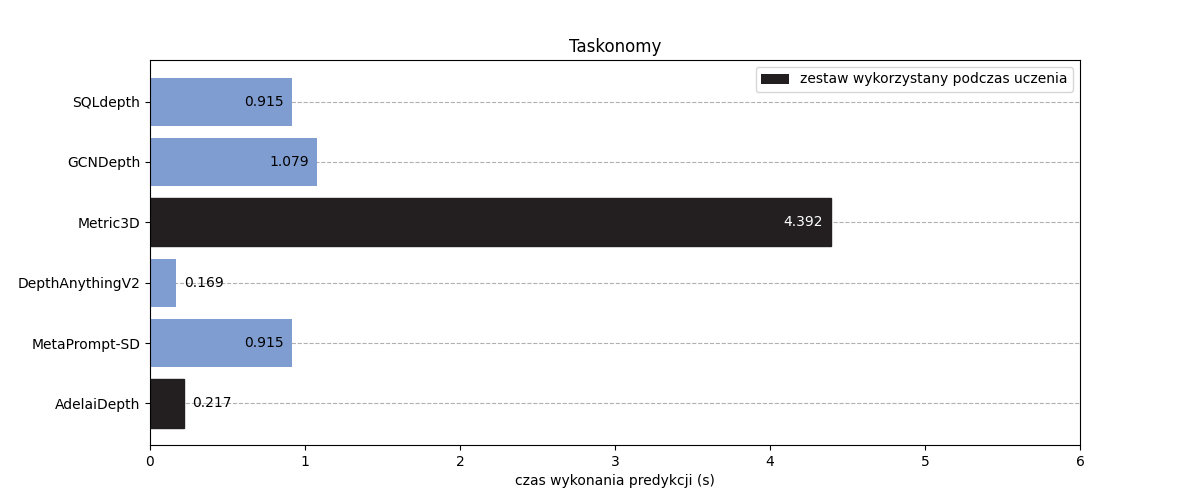
\includegraphics{plots/exec_time/6}
    \caption{Średni czas wykonania estymacji na zbiorze Taskonomy.}
    \label{fig:exec_time_6}
\end{figure}

\section{Wymagania systemowe}
W trakcie analizy algorytmów zostały zarejestrowane szczytowe wartości zużytych zasobów systemu komputerowego udostępnionego przez platformę Google Colab. W tym celu zostały wykorzystane wbudowane narzędzia analityczne platformy. Zapisane wartości uwzględniają pamięć o dostępnie swobodnym (RAM), pamięć karty graficznej (GPU RAM) oraz zajętość przestrzeni dyskowej (HDD). Najwyższa wartość w każdej z kolumn została oznaczona grubszą czcionką, druga najwyższa podkreśleniem.

\begin{table}[H]
    \centering
    \caption{Wykorzystane przez algorytmy zasoby komputerowe.}
    \vspace{0.1cm}
    \resizebox{\textwidth}{!}{%
        \begin{tabular}{ |p{3cm}|p{3cm}|p{5cm}|p{5cm}|r| }
        \hline
        Algorytm & RAM & GPU RAM & HDD \\
        \hline \hline
        AdelaiDepth &
        3,6 GB & 
        0,8 GB &
        4,7 GB \\
        \hline
        MetaPrompt-SD &
        \textbf{11,6 GB} & 
        \textbf{11,4 GB} &
        \textbf{27,7 GB} \\
        \hline
        Depth Anything V2 &
        4,9 GB & 
        6,5 GB &
        \underline{16,2} GB \\
        \hline
        Metric3D &
        \underline{5,7 GB} & 
        \underline{7,5 GB} &
        16 GB \\
        \hline
        GCNDepth &
        4,7 GB & 
        1,4 GB &
        7,6 GB  \\
        \hline
        SQLdepth &
        3,5 GB & 
        1,7 GB &
        15,1 GB  \\
        \hline
        \end{tabular}%
    }
    \label{tabela_wymagania}
\end{table}